\chapter{Background} \label{chp::bg}

For self-containedness, we provide a short reference to the mathematical tools
that we have been frequently used in PLVMs. Readers familiar with the theory of
conjugate duality and EM algorithm can skip the content of this chapter. And for
a comprehensive account, please refer to the book \cite{hiriart1993convex}.

\section{Conjugate Duality}

The conjugate in optimization context refers to the transformation of a problem
to another accompanying problem. The transformation is also known as the
\emph{conjugacy} operation or the \emph{Legendre-Fenchel} transformation.  It
plays an important role in the Lagrangian duality as well as the general convex
optimization. To start our discussion, we formally define the conjugate of a
function as:

\begin{dfn}

  The conjugate of a convex function~\footnote{we make a stronger assumption
  that $f$ is convex which can relaxed to the existence of a affine function
  memorizing $f$ on $\mathrm{dom}\, f$.} $f$ is the function $f^*$ defined by

  \begin{equation}
    f^*(s) = \sup \{ \langle s, x \rangle - f(x) \}, \quad
    \forall x \in \mathrm{dom}\, f
  \end{equation}

\end{dfn}


\begin{figure}[h!]
  \centering
  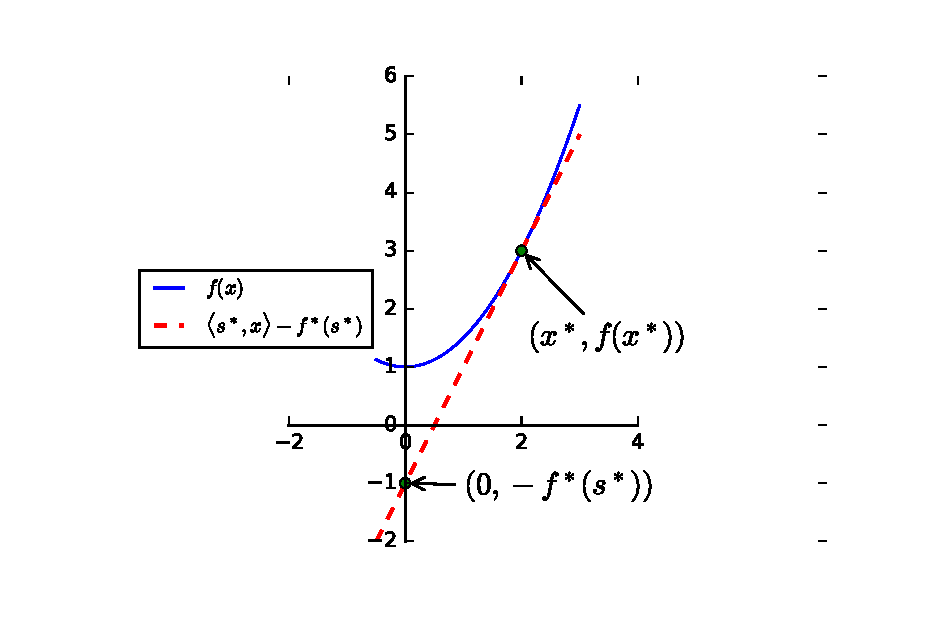
\includegraphics[width=0.7\linewidth, trim={0 0 3cm 1.5cm},
                    clip]{figures/conjugate-function.eps}

  \caption{A illustration of the relationship between $f$ and its conjugate
    $f^*$. For a given $s^*$, since $f(x) \geq \langle s^*, x \rangle  -
    f^*(s^*)$ always holds, which means that in the plot the curve of $f(x)$ is
    always above (or on) the line of $\langle s^*, x \rangle  - f^*(s^*)$. As a
    limiting case, $<s^*, x^*> - f^*(s^*)$ is cutting $f(x)$ at $x = x^*$. In
    addition, the affine function intersects the vertical axis $x = 0$ at the
    altitude $-f^*(s^*)$. The plot also shows the relationship between $s^*$ and
    $x^*$ can be described by the \emph{gradient mapping}: $x^* \in \partial
    f^{-1}(s^*)$, or equivalently $s^* \in \partial f(x^*)$.}

  \label{fig::conjugate-function}
\end{figure}

An geometrical interpretation of the conjugate of a \emph{subdifferentiable}
function is illustrated in \Cref{fig::conjugate-function}. A immediate
result is that:

\begin{thm} \label{thm::conjugate-attainer}
For any $x^* \in \argmax \{ \langle s^*, x \rangle  - f^*(s^*)
\}$, we have that $x^* \in \partial f^{-1}(s^*)$
\end{thm}

In addition, the conjugacy transformation is generally symmetric: $f^{**} = f$
for convex functions. To be exact, the identity between the bi-conjugate
$f^{**}$ and $f$ is equivalent to the requirement that the convex $f$ is lower
semi-continuity (l.s.c): $\liminf\limits_{x \rightarrow x_0} \geq f(x_0)$, a
sufficient condition of which is that $f$ is subdifferentiable.

\subsubsection{Log-Partition and Negative Entropy}

One important instance of the conjugate in PLVMs is between log-partition and
negative entropy, which are defined as:

\begin{alignat}{-1}
  &\text{Log-Parition:} & \quad
  A(\mathbf{x}) &= \log \sum\limits_{i = 1}^N \exp(x_i) \\
  &\text{Negative Entropy:} & \quad
  - H(\mathbf{p}) &= \sum\limits_{i = 1}^N p_i \log p_i
\end{alignat}
where $\mathbf{p}$ is an element in the simplex set which is defined as:
$$\Delta_N = \{\mathbf{p} \in
  \mathbb{R}^{N}: p_j \ge 0, \sum\limits_{j=1}^N p_j = 1\}$$

The log-partition function is often seen in Maximum Entropy models, energy-based
models, as well as Markov Random Fields, \etc. The straight-forward computation
involves a summation over $N$ items, which can be computationally challenging if
$N$ is large. For example, in Markov Random Fields, $N = m!$  where  $m$ is the
number of nodes in the random fields. Computing the log-partition function is
often the bottleneck for training such a model.

It is easy to verify that both functions are convex and smooth. Their connection
is presented in the theorem below.

\begin{lem} \label{lem::bk-cd}
  Assume that
  $$\P(i; \vs) = \frac{\exp(s_i)}{\sum\limits_{j=1}^N \exp(s_j)}$$
  and
  $$A(\vs) = \log \sum\limits_{j = 1}^N \exp(s_j)$$
  The conjugate duality between the log-partition function and negative entropy
  states:
  \begin{align}
    A(\vs) &= \max\limits_{\vmu \in \Delta_N}
                    \{ \sum\limits_{j=1}^N \mu_j s_j -
                       \sum\limits_{j=1}^N \mu_j \log \mu_j \} \nonumber \\
           &= \max\limits_{\vmu \in \Delta_N}
                    \{ \E_{\vmu} [s_j] + \entropy(\vmu) \} \label{eq::bk-cd}
  \end{align}
  where the maximizer is attained at:
  \begin{align}
    \mu_j^* = \P(j; \vs), \quad 1 \le j \le N \label{eq::bk-cd_sol}
  \end{align}
\end{lem}
\begin{proof}

  In light of \Cref{thm::conjugate-attainer}, the general proof of the
  conjugacy transformation between $f$ and $f^*$ is to verify that $x = \partial
  f^* \big( \partial f(x) \big)$. And it is easy to show that

  $$\vs = -\partial H \big(\partial A (\vs) \big)$$

  However, it is much more intuitive to alternatively prove by showing the
  equivalence in \Cref{eq::bk-cd}. We follow the derivation:

  \begin{align*}
    \E_{\vmu}[s_j] + \entropy(\vmu)
      &= -\sum\limits_{j=1}^N \mu_j \log \frac{\mu_j }{ \P(j; \vs) } +
          \log\sum\limits_{j=1}^N \exp(s_j) \nonumber \\
      &= -D_{KL}(\vmu || \P) + A(\vs)
  \end{align*}
  %
where $D_{KL}(\vmu || \P)$ is the Kullback-Leibler (KL) divergence.

Note that KL-divergence is always nonnegative:

$$D_{KL}(\vmu || P) \ge 0$$

and:

$$D_{KL}(\vmu || P) = 0  \quad\iff\quad \vmu = P $$

It follows that:

$$\vmu^* = \argmin\limits_{\vmu \in \Delta_N} D_{KL}(\vmu || P) = P$$

\end{proof}

\section{EM Algorithm: a modern reinterpretation} \label{sec::bg-em}

Equipped with the conjugate duality, here we offer a new interpretation of the
famous EM algorithm. Part of the idea presented here is also shared by the work
\cite{iusem1992primal}.

Suppose that there is a distribution $\P(Z | \Theta)$ where the data $Z = (X,
Y)$ is partially observed and can be decomposed into the observations $X$ and the
unseen variables $Y$. Given a set of data $X_1, \dots, X_N$, MLE solves the
problem:

$$ \max_\Theta \log \P(X_1, \dots, X_N | \Theta) $$

Using the conjugate duality proved in \Cref{thm::conjugate-attainer}:

\begin{align}
  \log \P(X_1, \dots, X_N ; \Theta) &=
\sum\limits_{i=1}^N \log \sum\limits_{Y_i} \P(X_i, Y_i ;\Theta)  \nonumber \\
&=
 \sum\limits_{i=1}^N \max_{\vmu_i \in \Delta} \Big(
  \sum\limits_{Y_i} \vmu_{i, Y_i} \log \P(X_i, Y_i ;\Theta) +
  \entropy(\vmu_i) \Big) \label{eq::em-conjugate}
\end{align}

Therefore, the MLE with incomplete observation amounts to:

$$
\max\limits_{\substack{\Theta \\ \vmu_i \in \Delta , 1 \leq i \leq N}}
\underbrace{\sum\limits_{i=1}^N  \Big(
  \sum\limits_{Y_i} \vmu_{i, Y_i} \log \P(X_i, Y_i ;\Theta) +
\entropy(\vmu_i) \Big)}_{\mathcal{F}(\Theta, M)} \nonumber
$$

And for fixed $\Theta$, the optimality condition for $\mu_i$ is:

\begin{flalign}
  &\text{E-step:} \quad \frac{\partial \mathcal{F}}{\partial \mu_i} = 0
\quad\iff\quad
\mu_{i, Y_i} = \P(Y_i | X_i; \Theta)
\end{flalign}
%
which is exactly the E-step in EM algorithm.

In addition, to optimize $\Theta$ while fixing $M$:

\begin{flalign}
  &\text{M-step:} \quad \max\limits_{\Theta}
\sum\limits_{i=1}^N \sum\limits_{Y_i} \vmu_{i, Y_i} \log \P(X_i, Y_i ;\Theta)
\end{flalign}

In the EM algorithm, $\sum\limits_{i=1}^N \sum\limits_{Y_i} \vmu_{i, Y_i} \log
\P(X_i, Y_i ;\Theta)$ is referred as \emph{evidence lower bound}~(ELBO)
function, and the above maximization is identical to the M-step in the EM
algorithm.

Using this interpretation, it is also straight-forward to view the EM algorithm
as a coordinate-descent algorithm where the objective function is constructed as
$\mathcal{F}(\Theta, M)$, which is always a lower bound of the log-likelihood.
In below, we briefly discuss two important variants of the EM algorithm.

\subsubsection{Variant 1: Relaxation by Approximation}

In the above basic version of EM, we assume that $\mu_i$ can freely choose any
element from the simplex $\Delta$. Nevertheless, it often posits a computational
difficulty when solving the posterior distribution $\P(\cdot | X_i; \Theta)$.
And it makes sense to trade accuracy of $\mu_i$ for computational efficiency,
and to compute an approximation of $\mu_i$ by a tractable surrogate, which
motivates us to study different approximation approaches in the variational
inference. In below, we discuss a few well adopted methods.

\noindent \textbf{Mean-Field Approximation}: The simplest strategy for
approximation is to restrict $\mu_i$ to be chosen from a subset, say,
$\mathcal{S}$ instead of $\Delta$. Then the optimization problem for $\mu_i$
with a constant $\Theta$ becomes:

\begin{equation}
\min\limits_{\mu_i \in \mathcal{S}} D_{KL}
\big(\mu_i \; ||\; P(\cdot | X_i; \Theta)\big)\label{eq::em-alg-e-appro}
\end{equation}

When $\P(\cdot | X_i; \Theta) \notin \mathcal{S}$, \Cref{eq::em-conjugate} will
not hold. In such cases, the solution of $\Theta$ will neither converge to that
of MLE.  Moreover, because of the restricted $\mu_i \in \mathcal{S} \subsetneq
\Delta$, the EM algorithm with mean-field approximation is in fact maximizing a
(strict) lower bound of the log-likelihood objective.

\noindent \textbf{Approximation by Sampling}: As discussed above, it is not
uncommon that the posterior $\P(\cdot | X, \Theta)$ does not yield a feasible
solution. However instead of compute the density analytically, it is generally
possible to use a Gibbs sampler to efficiently sample from the distribution. And
when incorporating such sampling-based E-step into the EM framework, it is
advantageous to run the Gibb sampler for only a few iterations (before its
converging) to collect the statistics for maximization in
M-step~\cite{wang2016tpp}, the idea of which can be justified similarly as that
of Contrastive Divergence~\cite{carreira2005contrastive}.

\noindent \textbf{General Density Approximation}: General methods for
approximation of $\P(\cdot | X, \Theta)$ digress from the optimization framework
of EM algorithm by substituting the objective of \Cref{eq::em-alg-e-appro} with
other forms of measurement for closeness. For example, Belief
propagation~\cite{yedidia2005constructing}, Bethe
approximation~\cite{burgess1978bethe} as well as expectation
propagation~\cite{minka2001expectation}, when used in EM do not yields a lower
bound nor upper bound of the log likelihood. Nevertheless, they are extensively
investigated for their empirical improvement in terms of efficiency and
performance. Especially, the expectation propagation~(EP) method was applied to
replace the E-step in the EM framework and it outperforms the mean-field
alternatives in cases when evidence is limited~\cite{wang2012truncation}. The EP
method can be viewed as an approximation to the minimization of the reversed
KL-divergence~\cite{minka2005divergence}:

\begin{equation}
\min\limits_{\mu_i \in \mathcal{S}} D_{KL}
\big(P(\cdot | X_i; \Theta) \; ||\;  \mu_i\big)\label{eq::em-alg-e-appro-rev}
\end{equation}

Comparing \Cref{eq::em-alg-e-appro-rev} to \Cref{eq::em-alg-e-appro}, we see
that the order of two distributions in the KL-divergence is reversed. The
in-depth discussion of this topic is beyond the scope of this thesis, and we
refer the readers to the brochure on variational
inference~\cite{wainwright2008graphical} and the Ph.D thesis of
\citet{minka2001family} on approximation in Bayesian inference for a
complementary review.

\subsubsection{Variant 2: Bayesian Variational Inference}

EM algorithm is also investigated in Bayesian setting although most techniques
remain the same. Specifically, $\Theta$ is viewed as a distribution which is
governed by hyperparameter $\Gamma$, and thus the log-likelihood function
involves not only marginalizing the latent variable $Y$ but also the parameter
$\Theta$.

In the Bayesian setting, EM is more often called as Bayesian variational
inference method. Mathematically, $\Theta$ is also a latent variable, no
different from $Y$, and we can still employ the EM algorithm. However, with
sufficient observations, the optimization of hyperparmeter $\Gamma$ is less
interested and the M-step is generally skipped. More importantly, by carefully
choosing the form of the prior distribution $\P(\Theta ; \Gamma)$ (as conjugate
prior of $\P(Y ; \Theta)$), we have the posterior $\P(\Theta | Y ; \Gamma)$ in
the same family of distributions as the prior. This is appealing since the
update of $\mu_i$ in \Cref{eq::em-conjugate} can be maximized exactly easily.

\section{Minimax Theory}

In this section we will review some results in the minimax theory which gives
the conditions under which the following equality is hold:

\begin{equation}
 \max\limits_{z \in Z} \min\limits_{x \in X} \phi(x,z) =
 \min\limits_{x \in X} \max\limits_{z \in Z} \phi(x,z)  \label{eq::minimax}
\end{equation}

\citeauthor{neumann1928theorie} is credited with the first investigation of this
problem.  There are many different sufficient conditions that guarantees the
above equation. Modern analysis employs Farkas Lemma in the \emph{min common/max
crossing} framework and an excellent formal discussion can be found in
\cite{bertsekas2003convex}. In this thesis, we only present an earlier version
of minimax theory by Sion~\cite{sion1958general}, which is one of several
celebrated generalizations of von Neumann's minimax
theorem~\cite{neumann1928theorie}:

\begin{thm}[Sion's Minimax Theorem]\label{thm::sion-minimax}
  Let $X$ and $Z$ both be a compact convex set. Let $\phi$ be a real-valued
  function on $X \times Z$ such that:
  \begin{enumerate}
    \item $\phi(x, \cdot)$ is upper semi-continuous and quasi-concave on $Y$ for
      any $x \in X$
    \item $\phi(\cdot, y)$ is lower semi-continuous and quasi-convex on $X$ for
      any $y \in Y$
  \end{enumerate}
  Then,
  $$ \max\limits_{z \in Z} \min\limits_{x \in X} \phi(x,z) =
     \min\limits_{x \in X} \max\limits_{z \in Z} \phi(x,z)  $$
\end{thm}

An elementary proof of Sion's minimax theorem can be found in
\cite{komiya1988elementary}. The derivation is simple, short and elegant. Also,
the assumption made in \cref{thm::sion-minimax} is often satisfied for most
practical problems under mild assumptions of $\phi$. In general,
\Cref{eq::minimax} holds when solving problems involving the dual formulation in
PLVMs.
